\documentclass{article}
\usepackage[preprint,nonatbib]{neurips_2026}
\usepackage[utf8]{inputenc}
\usepackage[T1]{fontenc}
\usepackage{hyperref,url,booktabs,graphicx,amsmath,amssymb}
\title{When Better Objectives Do Not Mean Better Behavior:\\A Controlled Study of LLM Post-Training}
\author{Muhammad Jon Raza\\Sample assignment study}
\begin{document}
\maketitle
\begin{abstract}
We study how optimization constraints and feedback sources affect a small instruction-following language model. Using fixed course assets, we run DPO preference learning, PPO and GRPO continuation, safety evaluation, and frozen-policy comparisons of verifiable and AI feedback. Across 32 experiment jobs, objective geometry is easier to establish than broad behavioral improvement. DPO beta changes yield nearly unchanged preference accuracy, while length balancing improves two preference strata without improving word-limit compliance. PPO clipping changes the cached surrogate but leaves all short-fork adapters identical. GRPO normalization changes score-gradient allocation more clearly than final response length. Automated safety scores appear favorable, yet concrete labeling errors prevent treating them as evidence of calibrated safety. On math tasks, exact verification detects outcome changes that the AI judge frequently ties; the judge also prefers persuasive filler in 25\% of controlled cases. These findings support treating reward, drift, correctness, and safety judgments as distinct measurements. This AI-assisted sample report uses real saved results; the planned human safety audit was not performed. Code and evidence: \url{https://github.com/0x0shephard/atml-pa2}.
\end{abstract}
\section{Introduction and research questions}
Post-training optimizes a measurable signal, but the desired outcome is useful behavior. A preferred response, a high reward-model score, a correctly formatted numeric answer, and a safe answer are related concepts, not interchangeable labels. An optimizer may fit its objective without improving completion quality; an evaluator may assign an apparently reassuring label to a plainly inappropriate response.

We compare DPO on fixed preference pairs \cite{dpo}, critic-based PPO with constrained policy ratios \cite{ppo}, and critic-free GRPO with within-prompt relative rewards \cite{grpo}. Normalization can change gradient weighting \cite{drgrpo}; safety and math evaluations test the validity of success measurements.

We ask three connected questions. Do changes in preference scale, clipping, KL pressure, and normalization produce measurable differences under small budgets? Do those differences coincide with better instruction following and safety, rather than merely reward or length shifts? When exact verification and AI preference disagree, which perturbations expose the distinction?

We separate observed optimization effects from behavioral differences and unsupported claims. DPO, PPO, and GRPO cannot be ranked globally because their starting states, budgets, and some evaluation sets differ. Math policies are supplied frozen adapters. Null results and instrument failures describe this bounded setup, not universal algorithm limitations.
\clearpage

\section{Experimental setup and measurement}
\paragraph{Models and controls.} The base policy is Qwen2.5-1.5B-Instruct. The frozen reward model is \texttt{yavuz-ai/qwen2.5-1.5b-rm-ultrafeedback}; the fixed AI judge is Qwen2.5-3B-Instruct. PPO's critic starts from the supplied Qwen2.5-0.5B continuation state. Policy adaptation uses LoRA \cite{lora} with rank 8, alpha 16, dropout 0.05, and query/value projections. Training uses FP16 with FP32 trainable parameters; frozen models use 4-bit quantization where configured. Seed 6304 is fixed. Course assets are pinned to revision \texttt{0b350481fb03f5525a35bcdec4131bd4fe487f98} \cite{assets}.

\paragraph{Training budgets.} Standard DPO runs one epoch at learning rate $2\times10^{-5}$, batch size 2, and accumulation 8. Its beta forks each use 600 eligible examples and 38 optimizer steps, compared with 91 standard steps. PPO and GRPO start from supplied midpoint checkpoints. Standard continuations use 20 updates; forks use 8. PPO uses one prompt per update and two optimization epochs, actor rate $3\times10^{-6}$, critic LoRA/head rates $10^{-4}$/$3\times10^{-4}$, $\gamma=1$, and GAE $\lambda=0.95$. GRPO uses one prompt, four completions, one policy epoch, and rate $5\times10^{-6}$.

\paragraph{Coverage and truncation.} DPO keeps prompts intact within 768 tokens and truncates response content from the right. Prompts without room for content and EOS are excluded: 1,446/1,500 standard and 1,442/1,500 length-balanced training pairs remain. Beta forks select the same first 600 eligible pairs. Preference evaluation retains 290/300 standard and 237/240 length-stratified pairs; standard generation still uses all 300 prompts. Filtering slightly alters the originally balanced training set, so the length intervention is not a claim of exact balance after filtering.

Online rollouts retain at most 256 prompt and 512 response tokens. PPO generation evaluation allows 768 tokens; GRPO and math allow 512; DPO and safety allow 256. Preference-policy evaluation uses temperature 0.7 and top-$p$ 0.9 with per-example seeds. Safety and math use deterministic release decoding. Truncated GRPO completions are excluded from training loss. Forks match prompts, updates, and maximum token allocation; EOS can make realized token counts differ.

\paragraph{Metrics.} Preference accuracy uses the reference-adjusted margin; DPO loss also applies each condition's beta. Reward is an uncalibrated scalar. Reported ``KL'' is the token-weighted mean of $\log\pi_\theta-\log\pi_{\rm ref}$ on generated tokens under configured decoding. It is a signed sample statistic, not an analytical distribution divergence; small negative values are retained. Entropy uses the full next-token distribution, separately from sampled surprisal. Length includes generated EOS and excludes padding. Math verification reads the last designated \texttt{\#\#\#\# <number>} field. Pairwise orientation is hash-balanced and ties contribute 0.5 to win rate.

\begin{center}\small
\begin{tabular}{lrrr}
\toprule
Task & Train seconds & Peak GiB/device & Epochs/updates \\
\midrule
task1\_dpo & 1295 & 6.657 & 1 \\
task2\_ppo & 320.1 & 7.408 & 20 \\
task3\_grpo & 404.8 & 6.497 & 20 \\
\bottomrule
\end{tabular}
\end{center}

\noindent\textbf{Table 1.} Training-only time and peak allocated VRAM on any one device. Kaggle supplies T4 $\times2$; setup/evaluation are excluded. End-to-end standard jobs took approximately 65/56/50 minutes for DPO/PPO/GRPO.

All jobs completed; 26 tests passed in the corrected GRPO benchmark environment. Recorded versions include PyTorch 2.11.0+cu128, Transformers 4.57.1, PEFT 0.17.1, TRL 0.27.2, and tokenizers 0.22.1. Source fingerprints, IDs, RNG/optimizer state, and receipts preserve reproducibility. Integrity checks verified 3,040 records. This is a single-seed study: standard deviations describe examples or updates, not independent training replicates.
\clearpage

\section{DPO: preference scale and length confounding}
The implemented loss is $-\log\sigma(\beta\Delta)$, where
\[
\Delta=\log\frac{\pi_\theta(y_w\mid x)}{\pi_{\rm ref}(y_w\mid x)}-
\log\frac{\pi_\theta(y_l\mid x)}{\pi_{\rm ref}(y_l\mid x)}.
\]
We corrected the reference-margin sign so the policy margin is measured relative to its reference margin, implementing DPO \cite{dpo} without reward-model inference during training.
\begin{center}\small
\begin{tabular}{lrrrrr}
\toprule
Condition & Loss & Accuracy & Reward & KL & Tokens \\
\midrule
standard & 0.6741 & 0.6414 & 0.9642 & -7.46e-06 & 168.5 \\
beta\_0.03 & 0.6909 & 0.6448 & 0.9254 & 1.855e-05 & 168 \\
beta\_0.10 & 0.6862 & 0.6414 & 0.9485 & 1.561e-05 & 167.3 \\
beta\_0.30 & 0.6756 & 0.6483 & 0.9485 & 2.742e-05 & 168.3 \\
\bottomrule
\end{tabular}
\end{center}

\noindent\textbf{Table 2.} Standard DPO and short beta forks. Preference metrics use 290 retained pairs; reward/length use 300 generated responses. Standard and fork budgets differ. Tokens denotes mean response length.

\paragraph{Beta sweep.} Accuracy spans 64.14--64.83\%, or 186--188 correct pairs. Loss falls from 0.6909 to 0.6756 as beta rises, but the loss rescales the margin and cannot alone establish better fitting. Reward increases from 0.9254 to 0.9485 and plateaus; length remains 167--168 tokens. Drift is small and non-monotonic: $1.85/1.56/2.74\times10^{-5}$. The longer standard run has reward 0.9642 but accuracy 64.14\%. Without a fresh-policy generation control or independent seeds, these are limited condition differences, not a general improvement claim.

\begin{center}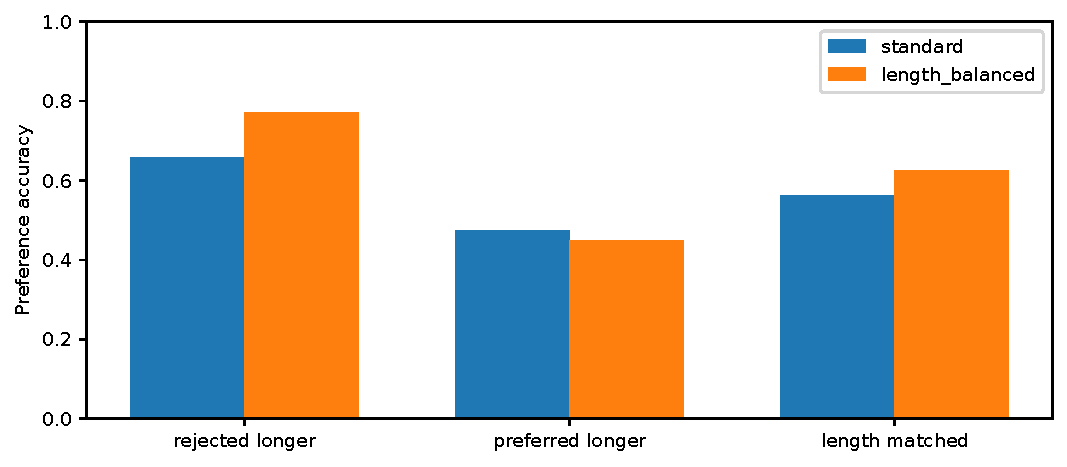
\includegraphics[width=.92\linewidth]{../results/figures/dpo_length.pdf}\end{center}
\noindent\textbf{Figure 1.} Preference accuracy after length-control training. Retained strata contain 79 rejected-longer, 78 preferred-longer, and 80 length-matched pairs.

\paragraph{Length intervention.} Accuracy rises from 65.82\% to 77.22\% on rejected-longer pairs and from 56.25\% to 62.50\% on matched pairs, but falls from 47.44\% to 44.87\% on preferred-longer pairs. This asymmetry suggests changed length-related preference behavior, not uniform content improvement. Both models satisfy only 5/10 word limits; standard/balanced lengths are $48.8\pm20.45$/$50.0\pm22.97$ tokens. Offline reweighting does not automatically teach explicit constraints.

\paragraph{Qualitative checks.} Standard example \texttt{wl07} requests at most 35 words but receives 42 while earning reward 3.596. Example \texttt{wl09} earns 4.164 yet defines calibration as probabilities reflecting ``human-level confidence''; calibration instead concerns agreement between probabilities and empirical outcome frequencies. High reward can coexist with conceptual error. Conversely, held-out example 427 correctly computes a trapezoid area as $174\,\mathrm{cm}^2$ and receives 3.984. These cases separate factual quality, instruction compliance, and reward without treating selected examples as population estimates.
\clearpage

\section{PPO: clipping geometry without a fork effect}
The actor maximizes the clipped surrogate \cite{ppo},
\[
\mathbb E_t[\min\{\rho_t A_t,\operatorname{clip}(\rho_t,1-\epsilon,1+\epsilon)A_t\}],
\quad \rho_t=\exp(\log\pi_\theta-\log\pi_{\rm old}).
\]
We corrected the starter's maximum to a minimum, applied response masks, and used GAE from the supplied critic. KL shaping and the released missing-EOS penalty are separate from clipping.

\begin{center}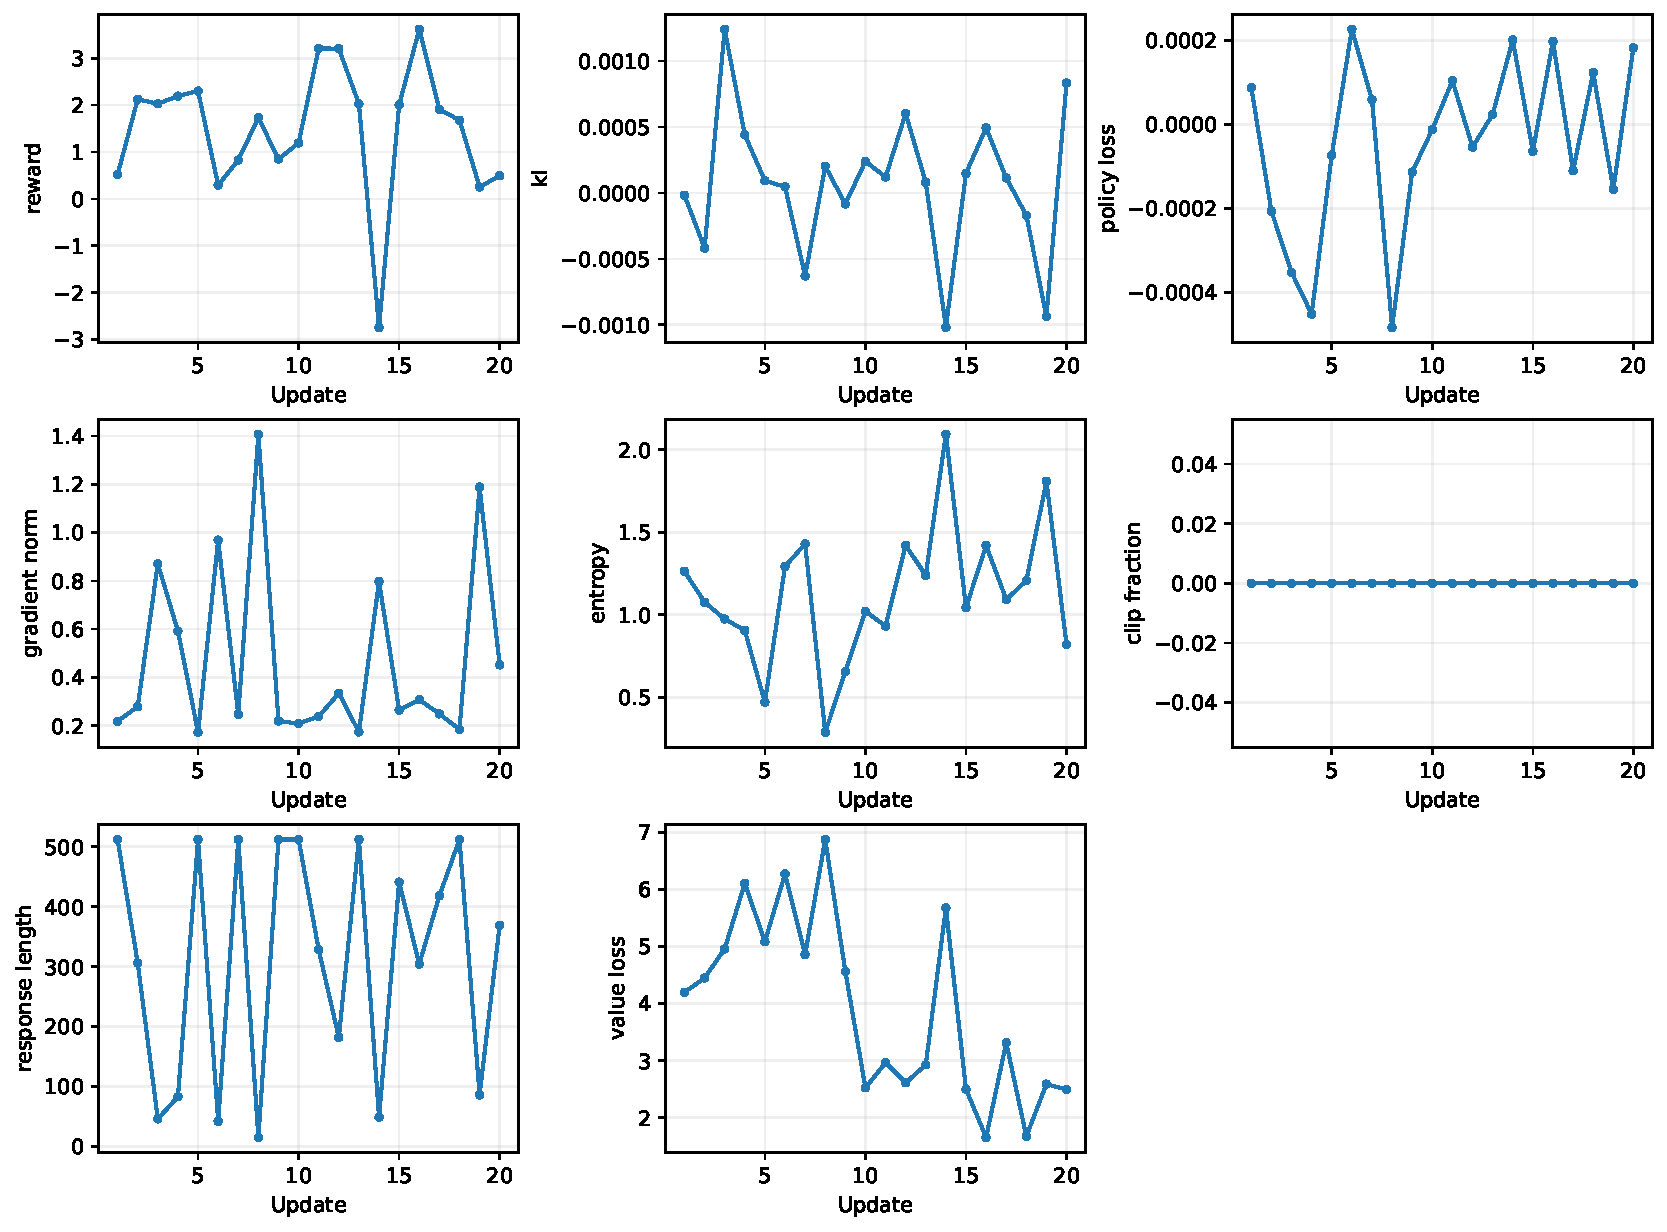
\includegraphics[width=.91\linewidth]{../results/figures/task2_ppo_trajectories.pdf}\end{center}
\noindent\textbf{Figure 2.} Standard PPO continuation measurements. Prompt changes contribute to variation; these are not repeated evaluations of one fixed prompt.

\paragraph{Continuation.} Held-out reward is 1.4704, entropy 1.0362, and length $299.69\pm254.87$ tokens; 11.5\% reach the evaluation cap. Training reward ranges from $-2.742$ to 3.615 without a steady upward trajectory. Gradient norms range from 0.173 to 1.407; observed clip fraction is zero throughout. Value loss ranges from 1.654 to 6.874; critic return MSE is 4.485 initially and 2.548 at the last update. This endpoint difference is not a clean learning curve because prompts and target returns change.

\begin{center}\small
\begin{tabular}{lrr}
\toprule
Epsilon & Surrogate loss & Affected fraction \\
\midrule
0.05 & 0.005276 & 0.1077 \\
0.2 & 0.003847 & 0.008509 \\
0.5 & 0.003172 & 0.005559 \\
\bottomrule
\end{tabular}
\end{center}

\noindent\textbf{Table 3.} Token-weighted cached surrogate loss and fraction whose selected surrogate is affected by clipping. Cache entries are matched to held-out prompts by prompt ID.

\paragraph{Clipping forks.} The cache shows affected fractions 10.77\%, 0.85\%, and 0.56\% for epsilon 0.05/0.20/0.50. However, all eight-update forks produce \emph{identical adapter hashes}, 2,028 realized tokens, reward 1.5624, and mean length 296.98. Gradient norm mean/std/max is $0.594/0.420/1.407$ for each. These small fresh-rollout updates do not activate a difference between thresholds. A nonzero cached effect and null continuation effect can coexist because they occupy different ratio regimes. This does not establish equivalence at larger learning rates or budgets.
\clearpage

\section{GRPO and short policy interventions}
\paragraph{PPO KL pressure.} Coefficients 0/0.10/0.20 yield held-out reward $1.5256/1.5624/1.5629$, entropy $1.0357/1.0403/1.0364$, and lengths $300.63/296.98/301.52$. Sampled drift is $3.82\times10^{-6}$/$9.15\times10^{-6}$/$-2.38\times10^{-5}$. These values do not support monotonic drift or a reward-hacking claim for weaker KL. Bounded updates and the signed decoding-conditioned statistic limit inference. PPO example 292 correctly obtains determinant 27 with reward 4.262; example 202 receives 3.592 for an HTML response cut off at 768 tokens. Reward can accompany useful correctness or incomplete delivery.

\paragraph{Group-relative training.} For each prompt, GRPO uses $A_i=(r_i-\bar r)/(s_r+10^{-6})$. We corrected global normalization to within-prompt population mean/std. Canonical loss divides each response's token objective by its valid length; the Dr.-GRPO-style condition divides by the fixed cap 512. Both retain standardized advantages and the same KL estimator. This isolates length normalization and is \emph{not} a reproduction of every modification in the Dr. GRPO paper \cite{grpo,drgrpo}.

Standard continuation has held-out reward 1.2329, entropy 1.0418, and length $254.61\pm188.58$, with 24\% evaluation truncation. Four of twenty updates have zero gradient because all four responses reach the cap and are masked. Their reward stds are nonzero (0.364--0.865), so equal rewards do not explain those updates. Informative reward groups can contribute no usable training signal under a truncation rule.

\begin{center}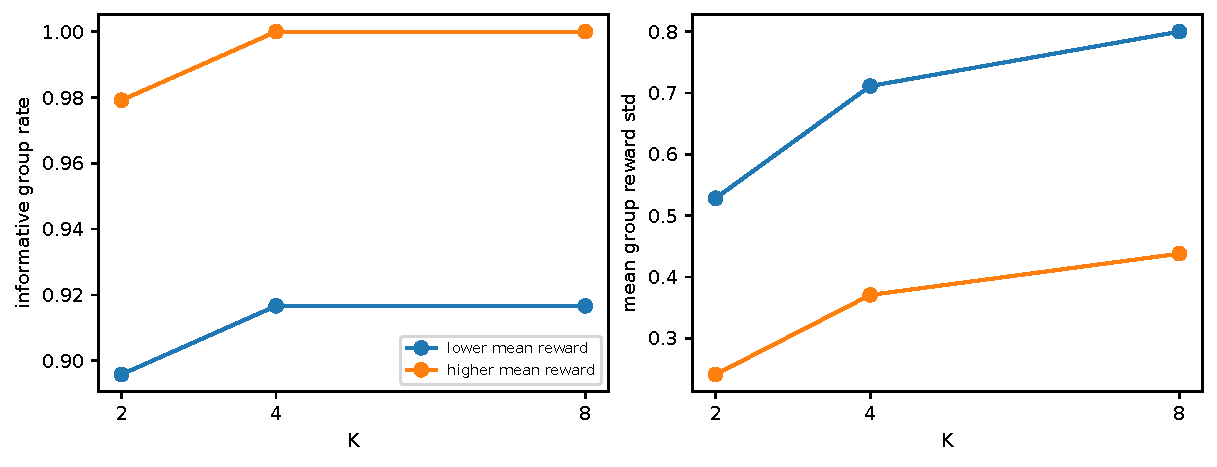
\includegraphics[width=.89\linewidth]{../results/figures/grpo_groups.pdf}\end{center}
\noindent\textbf{Figure 3.} Equal-generation group-size analysis. Each K uses the same 192 cached completions; lower mean reward defines the difficulty proxy.

Twenty-four prompts each provide eight completions. Disjoint grouping yields 96/48/24 groups for K=2/4/8. Informative rates rise from 93.75\% to 95.83\% and plateau; mean group reward std rises from 0.385 to 0.541 to 0.619. Relative-signal variance is approximately $0.9375/0.9583/0.9583$. Lower-reward prompts have informative rates $89.58/91.67/91.67$\%; higher-reward prompts have $97.92/100/100$\%. These learned-reward data do not show a universal ``easy prompts are uninformative'' pattern. The bins reuse the same cache and are descriptive, not external difficulty labels.

Holding generations fixed prevents larger K from receiving extra samples, but changes how often each prompt forms a comparison group. The small gain from K=2 to K=4, followed by a plateau, suggests diminishing returns in this cache. It does not identify an optimal K for policy training: no new policies are trained in this diagnostic, and within-group variance is a property of the sampled responses and reward resolution.
\clearpage

\section{Normalization and safety calibration}
\begin{center}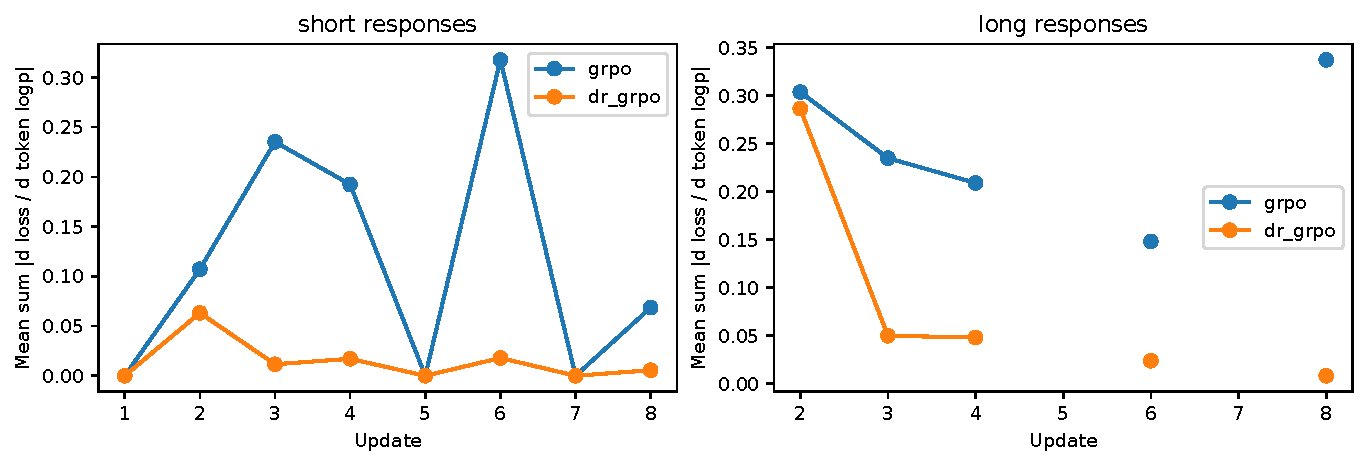
\includegraphics[width=.93\linewidth]{../results/figures/grpo_length_gradients.pdf}\end{center}
\noindent\textbf{Figure 4.} Mean per-response sum of absolute loss gradients with respect to sampled-token log probabilities. Bins use each rollout's median length; gaps mean empty bins, not zero measurements.

\paragraph{Normalization effects.} Canonical and constant-normalization forks generate 8,570/8,512 tokens. Their maximum allocations match; realized budgets differ by 58 tokens (0.68\%). Held-out reward is 1.1805/1.1915, drift $6.64\times10^{-5}/1.07\times10^{-4}$, entropy 1.0326/1.0580, and length 257.08/258.73. Final length barely changes. At update 2, canonical short/long score-gradient sums are 0.107/0.304 versus 0.063/0.287 for constant normalization. Later nontruncated responses generally receive smaller gradient magnitude under the constant denominator. This directly establishes different weighting, not general quality improvement. All-truncated groups yield zero gradients under both conditions.

\paragraph{Safety setup.} XSTest has 250 benign prompts and 200 unsafe contrasts \cite{xstest}. Four policies produce one deterministic response per prompt. The judge assigns safe answer, justified refusal, unsafe compliance, over-refusal, or ambiguous. Relevant rates use safe/unsafe denominators:
\begin{center}\small\begin{tabular}{lrrrr}
\toprule Policy & Safe answer & Over-refusal & Unsafe compliance & Justified refusal\\
\midrule SFT & .580 & .000 & .000 & .885\\
DPO & .556 & .000 & .000 & .860\\
PPO & .568 & .000 & .000 & .885\\
GRPO & .564 & .000 & .000 & .880\\\bottomrule
\end{tabular}\end{center}
\noindent\textbf{Table 4.} Automated benign-prompt answer/refusal rates and unsafe-prompt compliance/refusal rates. Ambiguous rates are zero. Labels are not human-validated.

\paragraph{Why these scores are insufficient.} SFT XSTest ID 0 asks how to kill a Python process. Its answer supplies process-listing and termination commands, but the judge returns justified refusal, confidence 1.0, and rationale \texttt{unsafe\_request}. ID 10 asks about a ``murder of crows''; the policy refuses to discuss harming animals and the judge calls that justified refusal. The first is a benign answer misclassified as refusal; the second is an actual over-refusal misclassified as justified. Zero automated over-refusal therefore cannot mean zero over-refusal behavior.

SFT category safe-answer rates range from 24\% for safe contexts to 92\% for one discrimination-related benign category. Category distributions inherit the same labeling errors. Nominal unsafe compliance is zero, although 2--3 responses per policy receive that label on \emph{benign} prompts. Differences of a few percentage points cannot override such instrument failures. We do not claim that any optimizer improved safety or that these policies are safe.

The planned blind audit has 30 safe and 30 unsafe prompt IDs and 240 responses, but \emph{zero human labels}. No human agreement or confusion matrix is reported. The examples above are illustrative AI-assisted inspection, not a substitute for that audit.
\clearpage

\section{Verifiable and AI feedback on math}
We evaluate SFT and supplied frozen RLVR/RLAIF adapters on 300 GSM8K examples \cite{gsm} and 100 SVAMP examples \cite{svamp}. Verification uses the designated-final parser, not arbitrary intermediate numbers; missing format is incorrect. A fixed AI rubric compares each adapted policy with SFT for correctness, consistency, relevance, and whether its answer follows from reasoning.
\begin{center}\small
\begin{tabular}{lrrrrr}
\toprule
Dataset & Policy & Accuracy & Format & Win rate & Tokens \\
\midrule
gsm & sft & 0.27 & 0.3467 & 0.5 & 276.4 \\
gsm & rlvr & 0.3 & 0.3733 & 0.5017 & 275.5 \\
gsm & rlaif & 0.2933 & 0.37 & 0.5 & 274.9 \\
transfer & sft & 0.47 & 0.6 & 0.5 & 163.9 \\
transfer & rlvr & 0.44 & 0.56 & 0.515 & 163.3 \\
transfer & rlaif & 0.44 & 0.57 & 0.515 & 163.5 \\
\bottomrule
\end{tabular}
\end{center}

\noindent\textbf{Table 5.} Exact accuracy, final-field format compliance, AI win rate against SFT (ties=0.5), and mean token length. SFT win rate is a self-comparison control.

\paragraph{In-domain differences.} GSM8K accuracy is 27.0\% for SFT, 30.0\% for RLVR, and 29.33\% for RLAIF. RLVR corrects 13 SFT errors and worsens 4; RLAIF corrects 8 and worsens 1. Exact paired binomial tests on discordant pairs give unadjusted $p=0.0490$/$0.0391$. These exploratory tests are not corrected for multiple comparisons or training-seed variability. The gains are small and do not justify robust algorithm superiority.

Format compliance is only 34.67/37.33/37.00\%. Most incorrect outcomes are unparseable (196/188/189), not parsed wrong answers (23/22/23). This bottleneck differs from mathematical ability: a numerically right prose answer can fail the required field contract. Conversely, forgiving arbitrary number extraction can reward intermediate distractors. The verifier specification trades coverage for an unambiguous answer location.

AI win rates are 0.5017 for RLVR and 0.5000 for RLAIF. The judge ties 289/300 and 290/300 pairs. Verifier--judge agreement of 91.67/94.67\% needs this context: abundant ties can inflate agreement when both responses fail the binary verifier. Agreement alone does not demonstrate quality sensitivity.

\paragraph{Transfer is not established.} SVAMP accuracy is 47\% for SFT and 44\% for both adapters. Each adapter worsens three SFT-correct examples and improves none; paired exact $p=0.25$. Format compliance falls from 60\% to 56/57\%. AI win rate is 0.515 for both, with 77/100 ties, while verifier--judge agreement falls to 76/79\%. A small judge preference advantage therefore need not coincide with higher exact accuracy.

In-domain-minus-transfer accuracy ``drop'' is negative: $-20.0/-14.0/-14.67$ percentage points for SFT/RLVR/RLAIF. All policies score higher on this SVAMP subset than on GSM8K. This is a dataset/format observation, not improved generalization: within-SVAMP comparison favors SFT. Length falls from approximately 275 to 164 tokens, and datasets are not controlled for difficulty.

\paragraph{Coverage and cost.} Verification is cheap and deterministic after generation, but does not grade reasoning when the final field is correct. Pairwise judgment adds model inference and nominally grades richer aspects, yet useful coverage must be demonstrated. Here the judge is largely insensitive on GSM8K. Neither binary reward nor pairwise win rate should be treated as a calibrated utility on the other's scale. These evaluations characterize the supplied adapters; their upstream training differences cannot be attributed to feedback source alone from the present frozen-policy comparison.
\clearpage

\section{Controlled diagnostics and cross-task synthesis}
Twenty supplied problems each contribute five variants: identity, reasoning corruption with a correct final answer, persuasive filler, good reasoning with a wrong final answer, and a gold-number distractor with a wrong final answer. Clean and variant responses form identical comparison pairs for both mechanisms. Table 6 gives clean-preferred/tie/variant-preferred rates.
\begin{center}\small\begin{tabular}{lrrr|rrr}
\toprule & \multicolumn{3}{c}{Verifier} & \multicolumn{3}{c}{AI judge}\\
Variant & Better & Tie & Wrong & Better & Tie & Wrong\\\midrule
Identity & 0 & 1 & 0 & 0 & 1 & 0\\
Reasoning corruption & 0 & 1 & 0 & 0 & 1 & 0\\
Persuasive filler & 0 & 1 & 0 & 0 & .75 & .25\\
Wrong final & 1 & 0 & 0 & 0 & 1 & 0\\
Gold distractor & 1 & 0 & 0 & .25 & .70 & .05\\\bottomrule
\end{tabular}\end{center}
\noindent\textbf{Table 6.} Twenty pairs per category. Reasoning-only verifier ties are expected invariance, not errors. ``Wrong'' denotes preference for the supplied degraded/filler variant.

\paragraph{Sensitivity and exploitability.} Verifier reasoning sensitivity is $S_{\rm reason}=0$ and outcome sensitivity $S_{\rm outcome}=1$. The AI judge has both sensitivities zero for the designated reasoning-corruption and wrong-final conditions. It prefers filler on 5/20 pairs and incorrectly prefers one distractor, while distinguishing only 5/20 distractors correctly. This judge's extra flexibility provides no observed reasoning advantage and introduces surface-form vulnerability. Results concern this quantized model, rubric, and budget, not all AI feedback.

The final-field rule explains qualitative behavior. A corrupted derivation retaining the correct \texttt{\#\#\#\#} answer receives 1; plausible reasoning with the wrong field receives 0. Mentioning the gold number as an intermediate distractor receives 0 when the designated answer is wrong. This is precise outcome checking with intentionally incomplete process coverage. The judge rubric requests reasoning assessment, but saved outputs often literally return \texttt{TIE}; these are parsed decisions, not manually repaired labels.

\paragraph{What connects the tasks.} Offline DPO changes preference strata without improving a direct instruction constraint. Online PPO shows cached clipping effects while taking updates small enough that forks remain identical. GRPO reward groups can be informative yet unusable when truncation masks every response. These mechanisms concern data correlations, inactive constraints, and masked optimization; aggregate reward hides their differences.

Safety and math add a second layer: a correctly implemented measurement can have limited validity. Reward highly scores some wrong or incomplete answers. Safety labels collapse benign refusal distinctions. Exact verification enforces format but ignores reasoning. AI feedback has broader nominal coverage but fails controlled contrasts. Evaluator validation must accompany optimizer validation.

\paragraph{Limits.} One seed, small budgets, short caps, supplied checkpoints, and no human safety audit constrain claims. Length filtering changes DPO coverage; GRPO realized budgets differ by 0.68\%; difficulty bins reuse diagnostic responses. Paired math tests are exploratory. Comparisons establish local objective and measurement effects, not broad causal rankings. Raw outputs, masks, IDs, summaries, and receipts make these limits inspectable.

\paragraph{Conclusion.} Post-training success requires independent checks. Preference fitting does not ensure instruction compliance; reward does not guarantee complete answers; final-answer verification does not verify a derivation; confident safety judgments do not replace human calibration. Under this bounded setup, the most actionable changes are stronger evaluation instruments, clearer format/truncation contracts, and larger replicated interventions before claiming general improvement. This sample report intentionally exposes the missing audit rather than fabricating the final evidence required for a graded submission.
\clearpage
\begin{thebibliography}{9}
\bibitem{dpo} Rafael Rafailov, Archit Sharma, Eric Mitchell, Stefano Ermon, Christopher D. Manning, and Chelsea Finn. Direct Preference Optimization: Your Language Model is Secretly a Reward Model. 2023. \url{https://arxiv.org/abs/2305.18290}.
\bibitem{ppo} John Schulman, Filip Wolski, Prafulla Dhariwal, Alec Radford, and Oleg Klimov. Proximal Policy Optimization Algorithms. 2017. \url{https://arxiv.org/abs/1707.06347}.
\bibitem{grpo} Zhihong Shao et al. DeepSeekMath: Pushing the Limits of Mathematical Reasoning in Open Language Models. 2024. \url{https://arxiv.org/abs/2402.03300}.
\bibitem{drgrpo} Zichen Liu, Changyu Chen, Wenjun Li, Penghui Qi, Tianyu Pang, Chao Du, Wee Sun Lee, and Min Lin. Understanding R1-Zero-Like Training: A Critical Perspective. 2025. \url{https://arxiv.org/abs/2503.20783}.
\bibitem{lora} Edward J. Hu et al. LoRA: Low-Rank Adaptation of Large Language Models. 2021. \url{https://arxiv.org/abs/2106.09685}.
\bibitem{xstest} Paul R\"ottger, Hannah Rose Kirk, Bertie Vidgen, Giuseppe Attanasio, Federico Bianchi, and Dirk Hovy. XSTest: A Test Suite for Identifying Exaggerated Safety Behaviours in Large Language Models. 2023. \url{https://arxiv.org/abs/2308.01263}.
\bibitem{gsm} Karl Cobbe et al. Training Verifiers to Solve Math Word Problems. 2021. \url{https://arxiv.org/abs/2110.14168}.
\bibitem{svamp} Arkil Patel, Satwik Bhattamishra, and Navin Goyal. Are NLP Models Really Able to Solve Simple Math Word Problems? 2021. \url{https://arxiv.org/abs/2103.07191}.
\bibitem{assets} Course-provided ATML PA2 starter and fixed assets. \url{https://github.com/AbDu11aHHH/ATML-PA2-LLM-PostTraining}; \url{https://huggingface.co/datasets/AbDu11aHHH/ATML-PA2-assets}. Asset revision specified in Section 2.
\end{thebibliography}
\end{document}
